\subsection{Security}
\begin{figure}[!htbp]
\centering
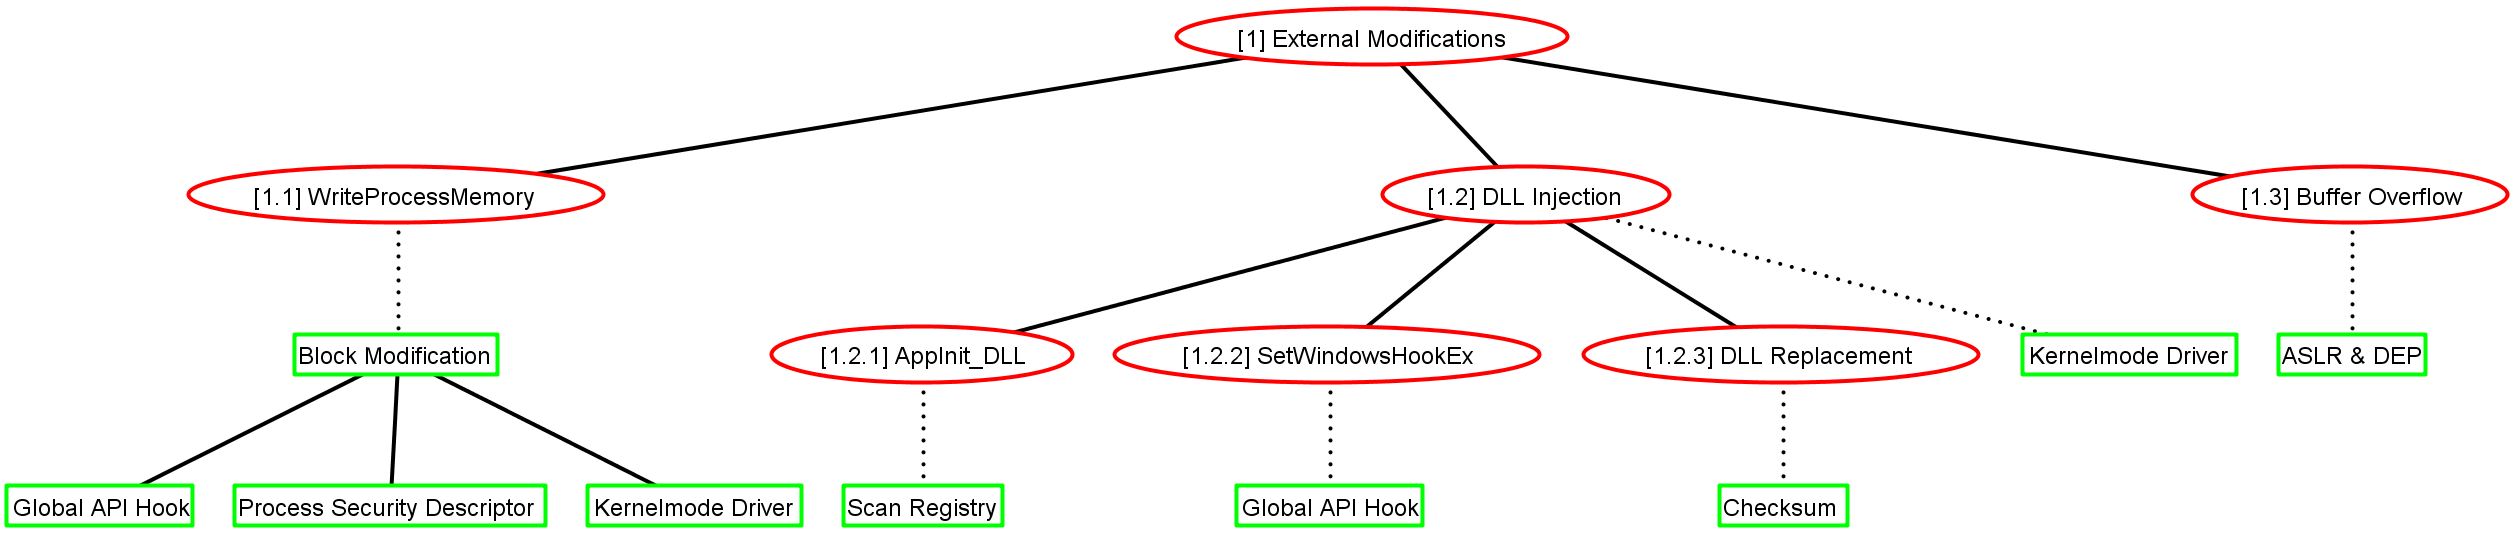
\includegraphics[angle=90,scale=0.3]{sections/adtrees/ExternalModifications.png}
\caption{The attack tree of Figure \ref{fig:attacks_external} with the added countermeasures}
\label{fig:attacks_external_def}
\end{figure}
The previously shown Figure \ref{fig:attacks} can be used as a basis for a security evaluation. To ensure that all attacks are no longer working, at least one countermeasure needs to be present, starting again with the external attacks of Figure \ref{fig:attacks_external}. The given \gls{WPM} call is blocked by the driver due to the \syscall{ObCallback} function. It is no longer possible to acquire a process handle with sufficient permissions and therefore all calls to \gls{WPM} will fail. Due to the drivers internal structure that keeps track of the created processes, it is possible to keep up the inter process communication between the chrome.exe processes. 

The second shown attack group, the \gls{DLL} injections which consists of several different ways, is blocked by the \syscall{PsSetLoadImageNotifyRoutine} callback. If a \gls{DLL} is about to be executed, its source file is hashed and compared to a whitelist. Only if a match is found, the execution is granted. Otherwise the \gls{DLL} is actively patched and no longer working. This callback function blocks the whole group of \gls{DLL} injections.

The third shown attack, the buffer overflows, have not been tackled by the driver. This is due to the nature of how buffer overflows work and the difficulty to detect them from a compiled program. In contrast to the first two attack groups, defenses are already existing and have been outlined in previous the Section \ref{sec:defenses}.

The result of these countermeasures and additional possible countermeasures can be seen in the updated attack defense tree in Figure \ref{fig:attacks_external_def}. This leaves the second way of modifications, the internal one still open. Figure \ref{fig:attacks_internal} showed the attack tree of the internal modifications. However, these ways are indirectly blocked by the external modifications. As the attacker is no longer able to get inside the target process, because all external modifications are no longer working, it is impossible to get an internal modification. Therefore, Figure \ref{fig:attacks_internal_def} shows the updated attack defense tree for internal modifications.
\begin{figure}[!htbp]
\centering
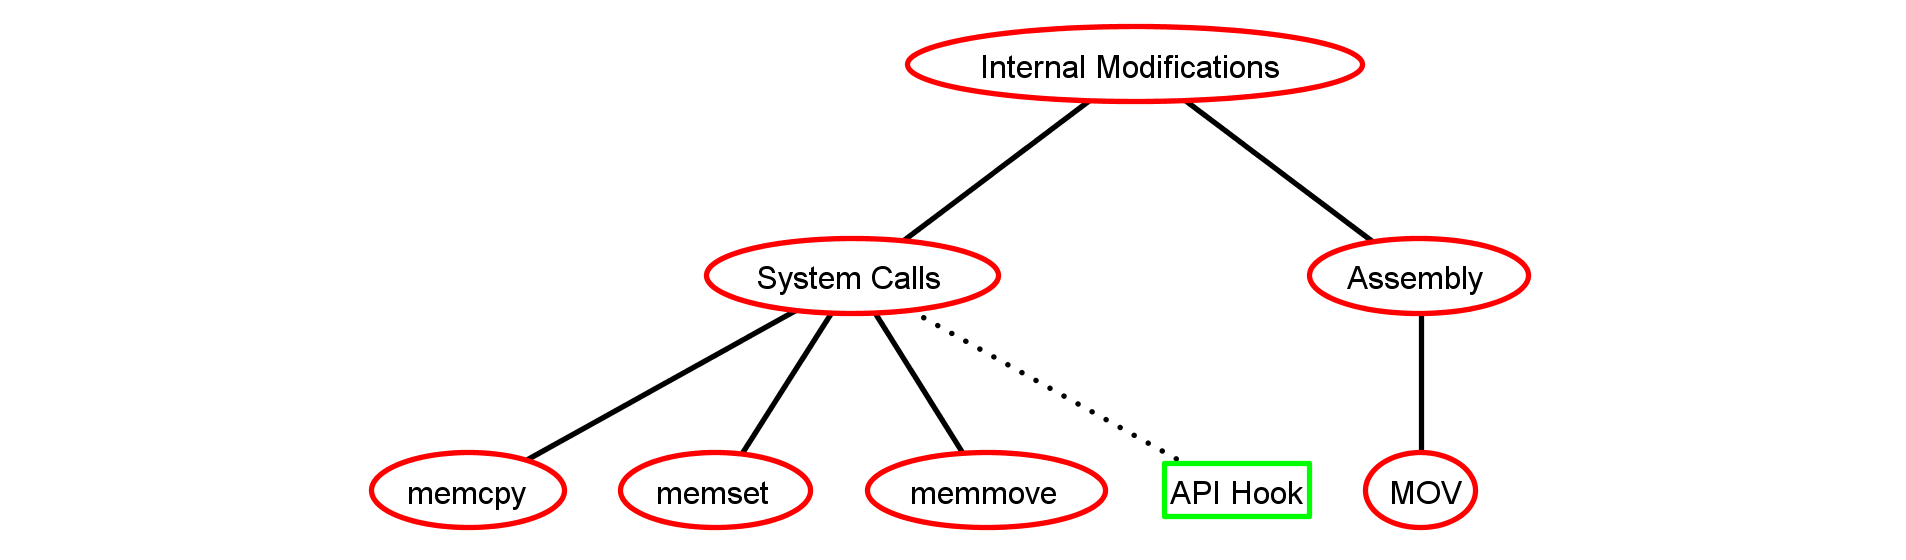
\includegraphics[scale=0.25]{sections/adtrees/InternalModifications.png}
\caption{The attack tree of Figure \ref{fig:attacks_internal} with the added countermeasures}
\label{fig:attacks_internal_def}
\end{figure}

To get a better understanding of the internal structures and resulting security of the driver and its weaknesses, a look at the three main parts, the process tree, the \gls{WPM} and the \gls{DLL} load component is taken.
To measure the security of \gls{WPM}, the underlying process tree structure needs to be looked at. 

A possible attack might make use of reusing a \gls{PID} that was assigned to a previously existing chrome process. The attacker might achieve this by flooding the system with many small processes, and by chance receiving the right \gls{PID} from the system. However, the attacker will not be able to fool the process tree structure, as exiting processes are removed and \gls{PID} reassignment therefore is not an issue. 

A second attack on the process tree might involve changing the attacking executable file name to chrome.exe, to be added to the list structure. Again, this will not grant the attacker any benefit. The tree maps child processes uniquely to a parent \gls{PID}. As both the fake and the real process are put into different list structures, they receive different outgoing pids. Therefore, no access is granted by the following \gls{WPM} call. In contrast to this attack, which changes the process name of the attacking executable, it is also possible to change the file name of the chrome process. This results in a case, that the driver can't detect and is one of the drivers limitation. This will lead to non existent protection on the renamed chrome process and therefore all given attacks continue working.

At last, the tree can't be changed from user mode, because the driver is running in kernel mode and user mode processes do not have access to the virtual memory of the driver. By that, the process tree structure can be considered as secure. This result directly leads to the security evaluation of the registered callback to prevent attacks via \syscall{WriteProcessMemory}. The permissions are by default removed, unless one of the following condition holds:
\begin{itemize}
\item Opened and Current process are equal, it is a self access
\item Opened and Current process \glspl{PID} are equal, it is a self access
\item Opened and Current process share the same \gls{PID} according to the process tree
\end{itemize}
The first two points are cases related to Chrome's inter process communication. They have to be allowed to keep Chrome working. The third point forces the driver to check the existing process tree structure. The results of a \syscall{FindPidInTree} call, located in Code Listing \ref{code:ptree.c}, on opened and current process need to be equal, or otherwise access can not be granted. Due to the fact, that the process tree structure has already been evaluated and was considered secure, \gls{WPM} is also blocked in all not allowed cases. 

Finally the third part has to be evaluated to make sure that all previously mentioned attacks will be prevented. As \syscall{PsSetLoadImageNotifyRoutine} is called whenever a \gls{DLL} was mapped into virtual memory and suspending the process, no execution can occur until the callback has finished. With respect to generating the required sha256 hash, the driver is very restrictive and if a required function call fails, access is denied. Only in cases where a matching entry inside the whitelist is found, access is granted. Therefore, \glspl{DLL} not on the whitelist will get blocked in all other cases. Because of that, any of the previously mentioned attacks like \gls{DLL} injection or using \syscall{SetWindowsHookEx} will no longer work. As a result, the driver can be considered secure and code injection attacks are successfully prevented.